\documentclass[11pt]{article}
\usepackage{setspace}
\usepackage{perpage}
\MakePerPage{footnote}
\usepackage[pdftex]{graphicx}
\usepackage{fullpage}
\usepackage{graphicx}
\usepackage{graphics}
\usepackage{psfrag}
\usepackage{pgf}
\usepackage{color}
\usepackage[latin1]{inputenc}
\usepackage[official]{eurosym}
\usepackage{amsthm}
\usepackage{amsmath,amssymb}
\usepackage{enumerate}
\setlength{\textwidth}{6.5in}
\setlength{\textheight}{8.5in}
\newcommand{\tr}{\textrm}
\title{$ $\\$ $\\ CSCI 678: Statistical Analysis of Simulation Models \\ $ $\\Final Project\\ $ $ \\Mid-Square Methods of Random Number Generation\\$ $ \\ $ $\\$ $ \\ $ $\\$ $ \\ $ $\\$ $ \\ $ $\\$ $ \\ $ $\\$ $ \\ $ $ \\$ $ \\ $ $ \\}
\date{April 29, 2014}
\author{Robert Johns}

\begin{document}

\pagenumbering{gobble}

\clearpage

\thispagestyle{empty}

\maketitle

\clearpage

\pagenumbering{arabic}
\tableofcontents

\clearpage

\doublespacing

%%%%%
%1
\section{Introduction}

$ $

The second sentence of the Wikipedia article for the mid-square method of random number generation states that it is ``not a very good method" for various reasons.  In this paper, the mid-square method is developed to the point where the second sentence of said article could state that it is ``a decent method" at minimum.

The mid-square method originated between 1240 and 1250 in a manuscript by a Franciscan friar known as Brother Edvin, possibly making it one of the first pseudorandom number generators described.  In 1949, Jon von Neumann gave a well-remembered talk on the mid-square method describing its flaws and stated that ``any one who considers arithmetical methods of producing random digits is, of course, in a state of sin".  While the mid-square method is indeed flawed in its initial construction, the most widely-used family of random number generators, Lehmer LCGs, are also arithmetic and to my knowledge, proprietors of such algorithms are not burning in any sort of hellfire.  So perhaps Jon von Neumann's dismissal is due for a reevaluation.

%%%%%
%2
\newpage
\section{The Mid-Square Method}

$ $

The algorithm for the mid-square method is as follows: take a four-digit random number and square it to get an eight-digit number; if fewer than eight digits result, add leading zeros to obtain eight total digits.  Take the resulting number and remove the first two and the last two digits to obtain a new four-digit number.  Repeat the algorithm with the resulting number to create a new random number.  Pseudocode for the algorithm follows:

To generate \texttt{MAX} variates:

$\texttt{count } \leftarrow 0$

$\texttt{while count < MAX:}$

$\hspace{1cm}\texttt{x}_1 \leftarrow \texttt{a}_1\texttt{a}_2\texttt{a}_3\texttt{a}_4$

$\hspace{1cm}\texttt{x}_2 \leftarrow \texttt{x}_1^2$

$\hspace{1cm}\texttt{x}_1 \leftarrow \lfloor \texttt{x}_2 / 100\rfloor \texttt{ mod } 10,000 \equiv \texttt{a}_{5}\texttt{a}_{6}\texttt{a}_{7}\texttt{a}_{8}$

$\hspace{1cm}\texttt{count}++$

$\texttt{end while}$


One notices several immediate benefits and problems with this algorithm.  One good thing is that it's simple to understand and straightforward to implement.  Another is that it's fast; very few operations are necessary to generate a variate, and because so few digits are required (only eight), modern processors have no trouble doing arithmetic at that level.

On the other hand, the algorithm has some serious issues. First and foremost, in this implementation, a maximum of four digits of precision is attainable.  Second of all, after several runs, a few statistical problems become apparent.  First of all, eventually all sequences degenerate to 0, almost always within the first 100 variates; whenever a seed is of the form ($00a_1a_2$), every subsequent variate will decrease.  Also, if a variate arises of the form ($a_1a_200$), every subsequent variate will be of that form, and the pattern will have a very short period.  Two examples follow to illustrate these shortcomings.

\newpage

Example 1: Generating 100 variates with seed 1234 (code: \texttt{om.c})

Results:

$$\begin{array}{|c|l|}\hline
\texttt{1 : 1234} & \texttt{54 : 3317}\\\hline
\texttt{2 : 5227} & \texttt{55 : 24}\\\hline
\texttt{3 : 3215} & \texttt{56 : 5}\\\hline
\texttt{4 : 3362} & \texttt{57 : 0}\\\hline
\texttt{5-53 : ...} & \texttt{58-100 : 0}\\\hline
\end{array}$$

Here we see examples of the first type of the first type of degenerate behavior; we get 56 relatively uniformly-distributed variates followed by an infinite string of zeroes with no way out of the loop.

\vspace{1cm}

Example 2: Generating 100 variates with seed 4564 (code: \texttt{om.c})

Results:

$$\begin{array}{|c|c|}\hline
\texttt{1 - 4564} & \texttt{5 - 4100}\\\hline
\texttt{2 - 8300} & \texttt{6 - 8100}\\\hline
\texttt{3 - 8900} & \texttt{7 - 6100}\\\hline
\texttt{4 - 2100} & \texttt{8 - 2100}\\\hline
\end{array}$$

Here we see the second type of behavior; the sequence quickly falls into a repetitive pattern with a period of 4.

%%%%%
%3
\newpage
\section{Improvements}

$ $

So far we have encountered three problems: lack of precision, convergence to 0, and short-periodic behavior with terms that are multiples of 100.  We can divide these issues up into two categories: the former containing the first issue and the latter containing the second two.

I contend that there are enough easy fixes to make the first issue not worth worrying about.  One simple fix would be to simply add more digits into the calculation; that is, square a six-digit number instead of a four-digit number.  As long as we remain within the bounds of integer overflow, this will work.  However, if we wanted more digits of precision than the processor could perform arithmetic with, another solution would be to generate two four-digit variates $x_1$ and $x_2$ and combine them into one eight-digit variate $x_1x_2$.  This gives us eight-digit precision with very little arithmetic cost, though it does cost us synchronization as we need two variates to make one.

The latter two issues are more worrisome.  However, a few simple edits can alleviate some of our worries and stay true to the spirit of the mid-square method.  Let's focus on the first issue, the convergence to 0.  We know that the problem arises because a variate is too small, which causes the next variate to be small, and so on, but we are unable to edit any given variate without disrupting randomness; if we had a variate of the form $a_1a_2a_3a_4$ where $a_1=a_2=0$, we would need to edit $a_1$ and $a_2$ to ensure that neither is 0.  However, if we do that, we disrupt the randomness and we would have no variates between 0 and 0.1.  We need a way to eliminate the degenerate behavior without editing the actual data of the individual variates.

Let's try an addition to our original algorithm.  Instead of just working from a variate $x = a_1a_2a_3a_4$, let's draw integers from sequences $s_1, s_2, s_3, s_4$ and append them to $x$ as follows: $\\x=b_1b_2a_1a_2a_3a_4b_3b_4$, where $b_i$ is drawn from $s_i$.  Then we square $x$ and take the middle four digits of $x^2$ as our new variate, and repeat.  Without directly changing $x$, we have ensured that $x$ cannot degenerate.  In our first run with this new algorithm, we see that the generator does not, in fact, converge to 0\footnote{Huzzah!}.  However, as illustrated in the following example, there is some disturbing behavior.

\newpage

Example 3: generating 10,000 variates with an initial seed of 4564. (code: \texttt{nm1.c})

Mean: 0.4779014, variance: 0.07546942, max: 0.9995, min: 0.0124

\begin{figure}[ht]
\begin{minipage}[b]{0.45\linewidth}
\centering
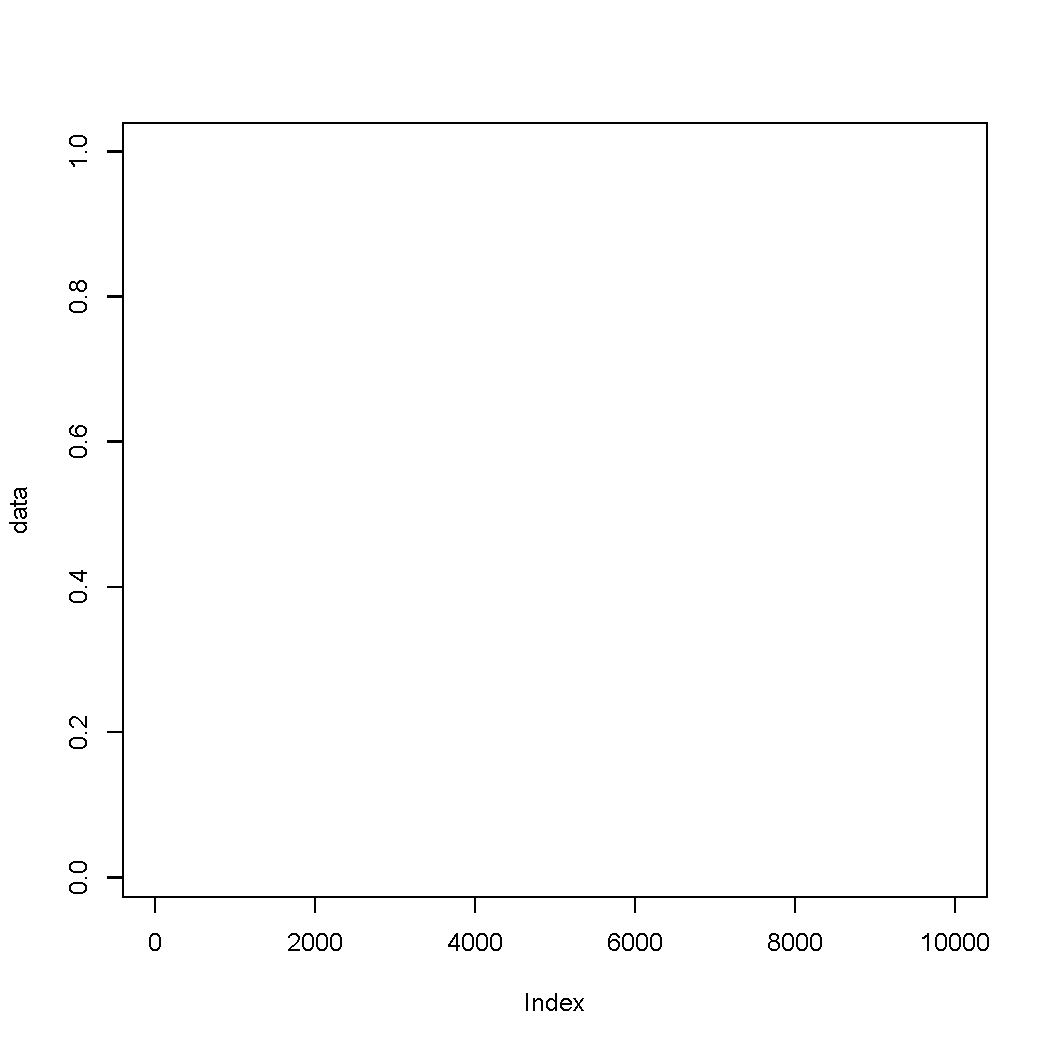
\includegraphics[scale=.42]{a4564raw.pdf}
\caption{Raw data}
\label{fig:figure1}
\end{minipage}
\begin{minipage}[b]{0.45\linewidth}
\centering
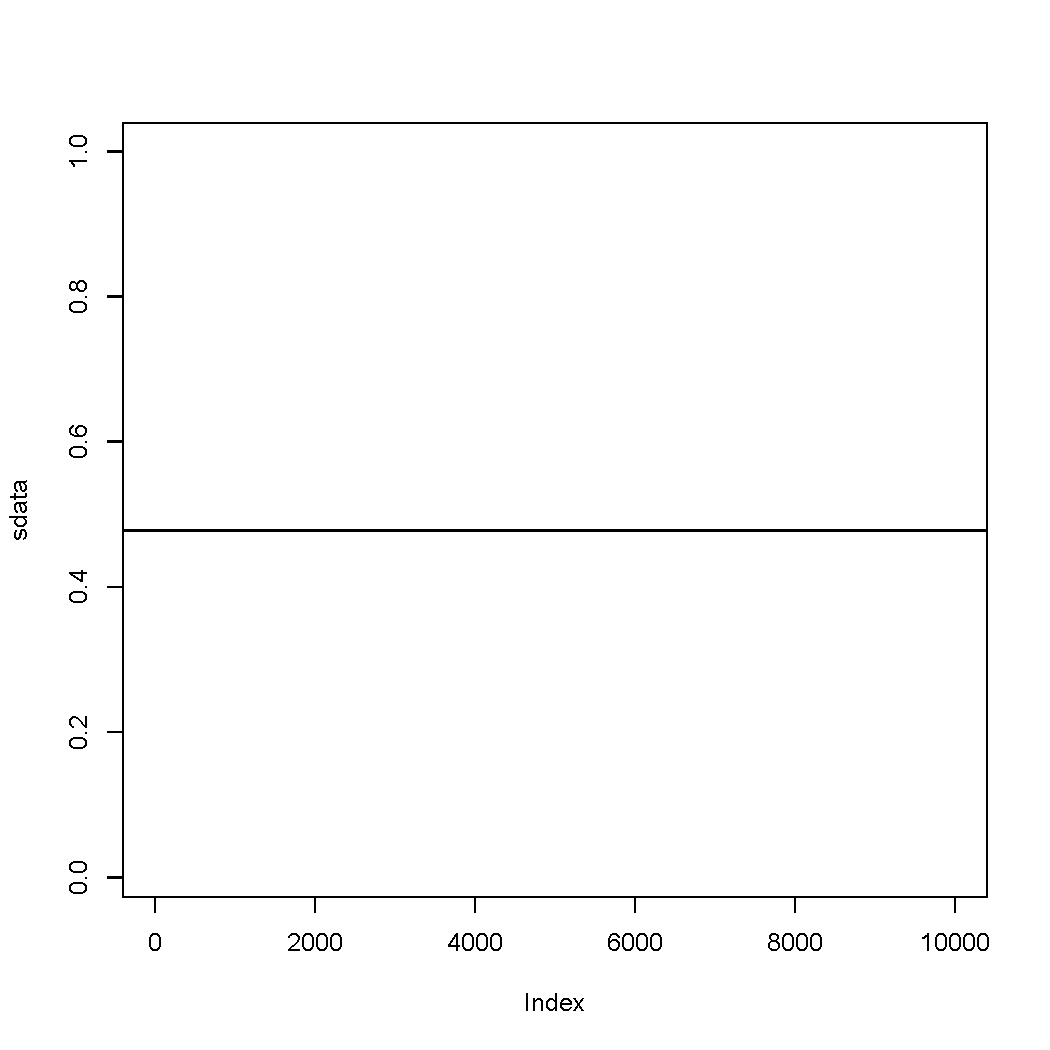
\includegraphics[scale=.42]{a4564cdf.pdf}
\caption{CDF with mean line}
\label{fig:figure2}
\end{minipage}

\begin{minipage}[b]{0.45\linewidth}
\centering
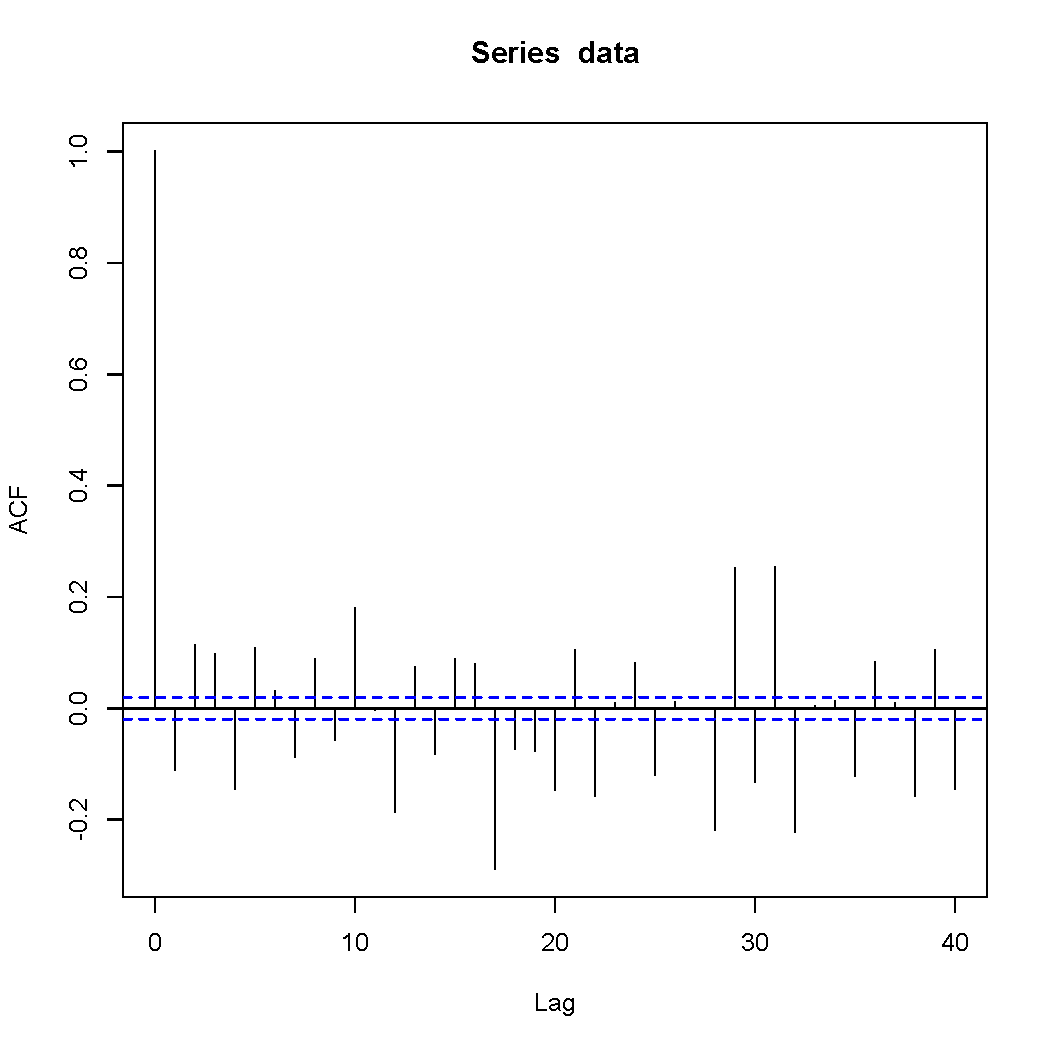
\includegraphics[scale=.42]{a4564acf.pdf}
\caption{ACF}
\label{fig:figure3}
\end{minipage}
\begin{minipage}[b]{0.45\linewidth}
\centering
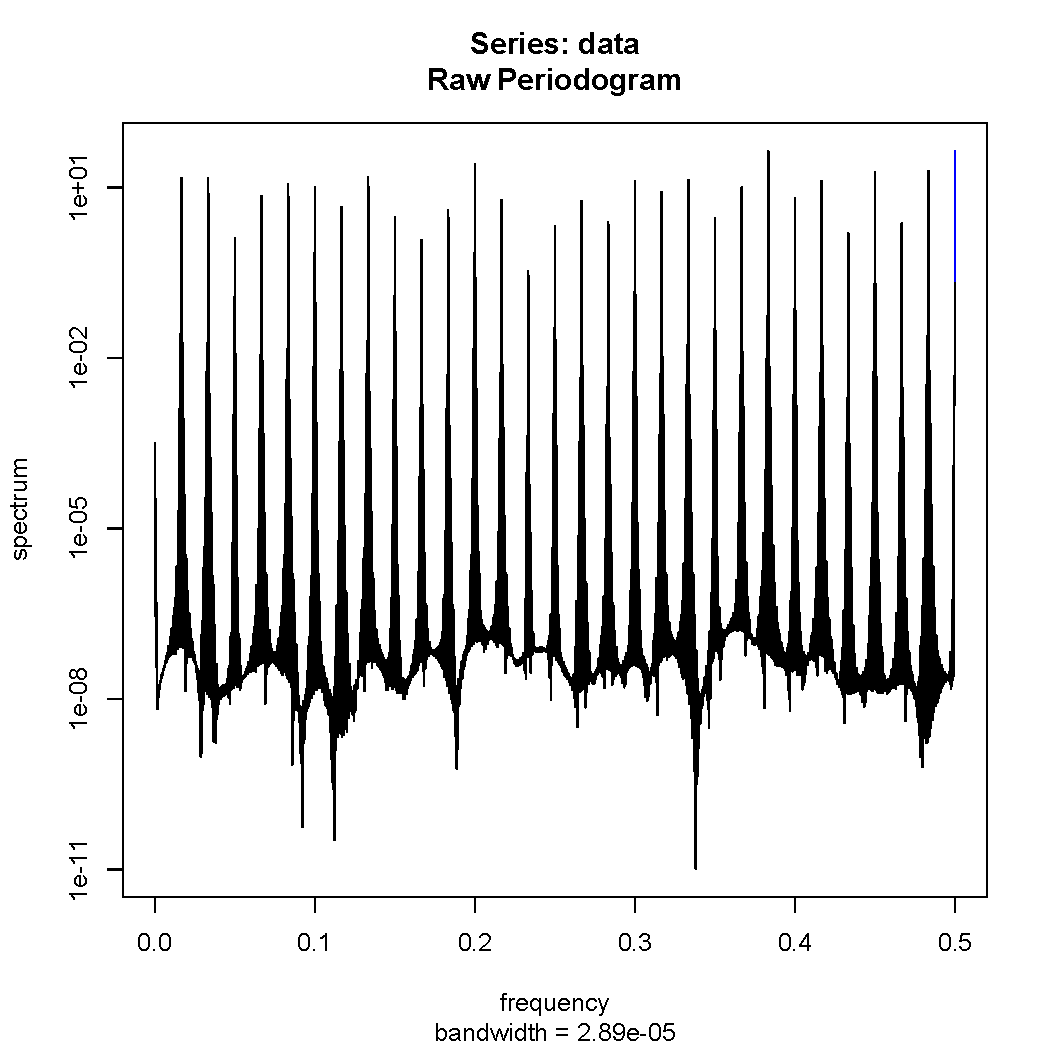
\includegraphics[scale=.42]{a4564pgram.pdf}
\caption{Periodogram}
\label{fig:figure4}
\end{minipage}
\end{figure}

The sequences used were:

\begin{verbatim}s1 = {7, 3, 2, 5, 4, 8, 9, 0, 1, 5}, s2 = {4, 2, 7, 9, 5, 0, 6, 2, 3, 1}
s3 = {5, 7, 4, 9, 8, 6, 2, 0, 1, 3}, s4 = {1, 7, 9, 5, 2, 3, 2, 8, 4, 6}\end{verbatim}

\newpage

So that wasn't very good.  Aside from the mean and variance being in the correct ballpark and the periodogram looking super awesome\footnote{Seriously, that's a cool-looking graph.}, not much good happened in the first example. We see that almost the entirety of the raw data falls on one of a few dozen lines, and there are disturbing jumps in the CDF, especially around the mean.  The autocorrelation function has large spikes around lag 30, and in almost all places is outside the confidence interval.  The periodogram indicates very periodic behavior consistently throughout the sequence.  However, in fixing our first issue, the degenerate-ness of the sequence, we have also fixed the second issue, the convergence to short periods of multiples of 100.  So that's something.

In order to fix the periodic behavior of the new generator, let's examine where such periodic-ness can arise.  One possibility is that it's fundamentally ingrained in the arithmetic of the method, but that's a depressing prospect so let's ignore it.  Another possibility is that the sequences from which the edited numbers were picked all had the same length (10).  We can easily fix this by editing the sequences so that they have lengths that are mutually coprime.  That way, the cycles of $b_1b_2\ldots b_3b_4$ would have period $|s_1|\cdot|s_2|\cdot|s_3|\cdot|s_4|$, where $|s_i|$ is the length of sequence $s_i$, as opposed to having period 10.  In the next example, we examine the results of our algorithm when we edit the sequences $s_1, s_2, s_3$ and $s_4$.

\newpage

Example 4: generating 10,000 variates with an initial seed of 4564 (code: \texttt{nm2.c})

Mean: 0.49923, variance: 0.08243094, max: .9999, min: .0002


\begin{figure}[ht]
\begin{minipage}[b]{0.45\linewidth}
\centering
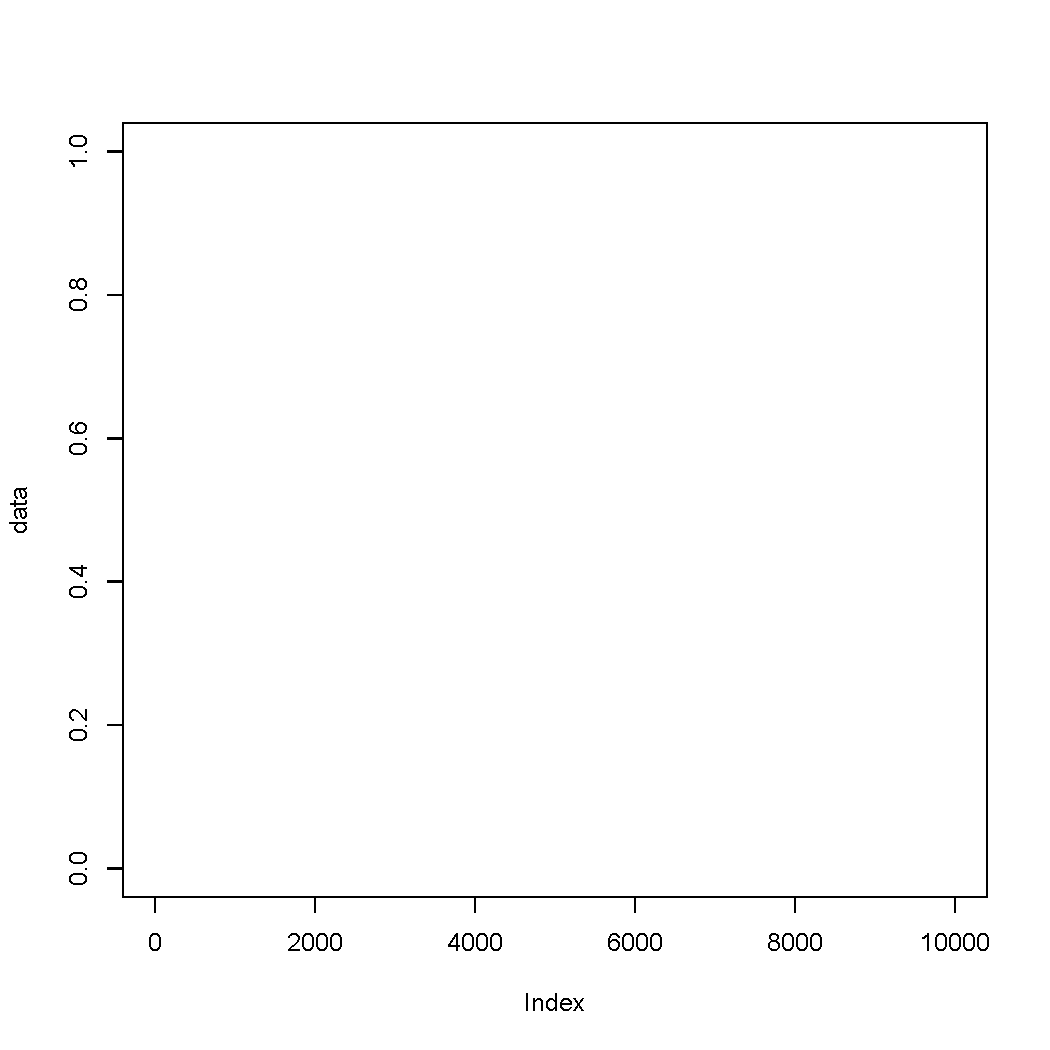
\includegraphics[scale=.42]{b4564raw.pdf}
\caption{Raw data}
\label{fig:figure5}
\end{minipage}
\begin{minipage}[b]{0.45\linewidth}
\centering
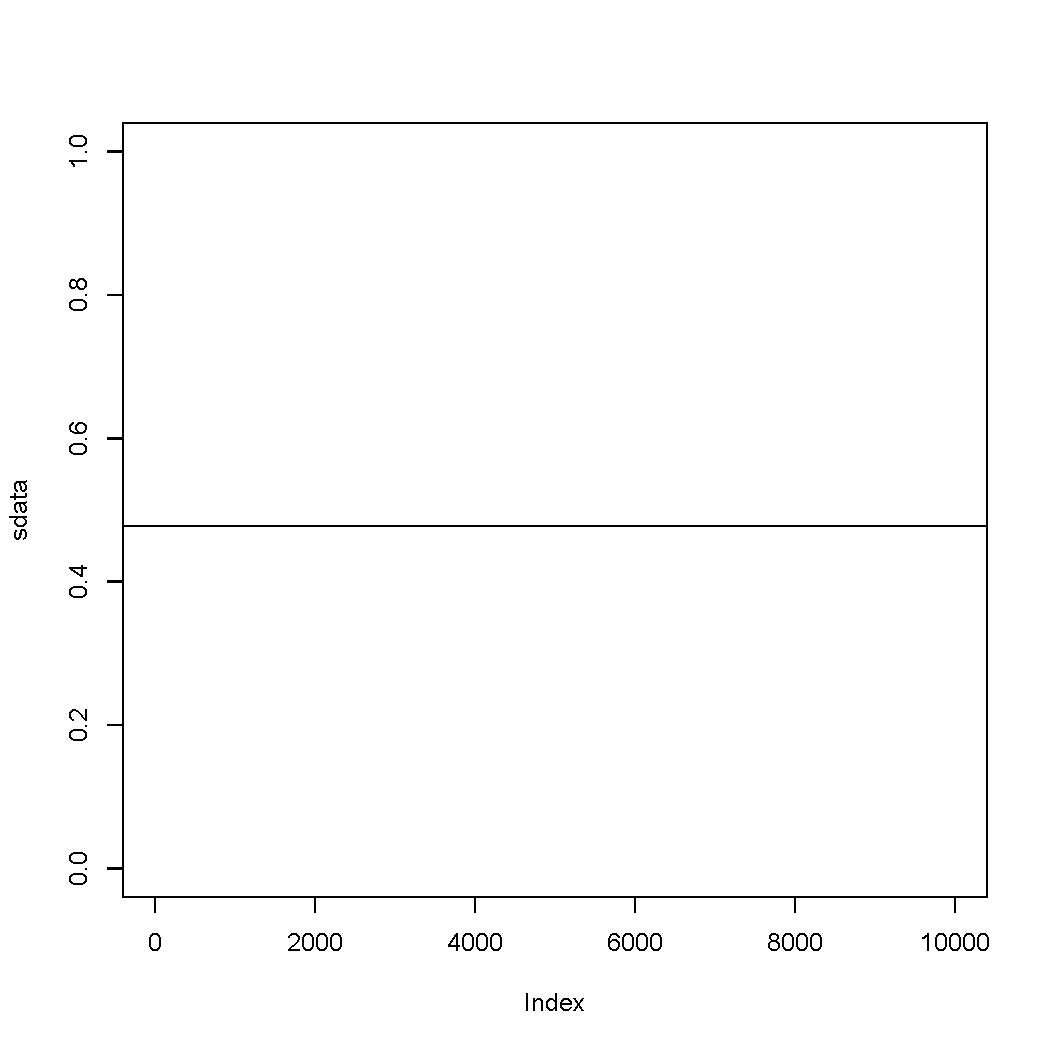
\includegraphics[scale=.42]{b4564cdf.pdf}
\caption{CDF with mean line}
\label{fig:figure6}
\end{minipage}

\begin{minipage}[b]{0.45\linewidth}
\centering
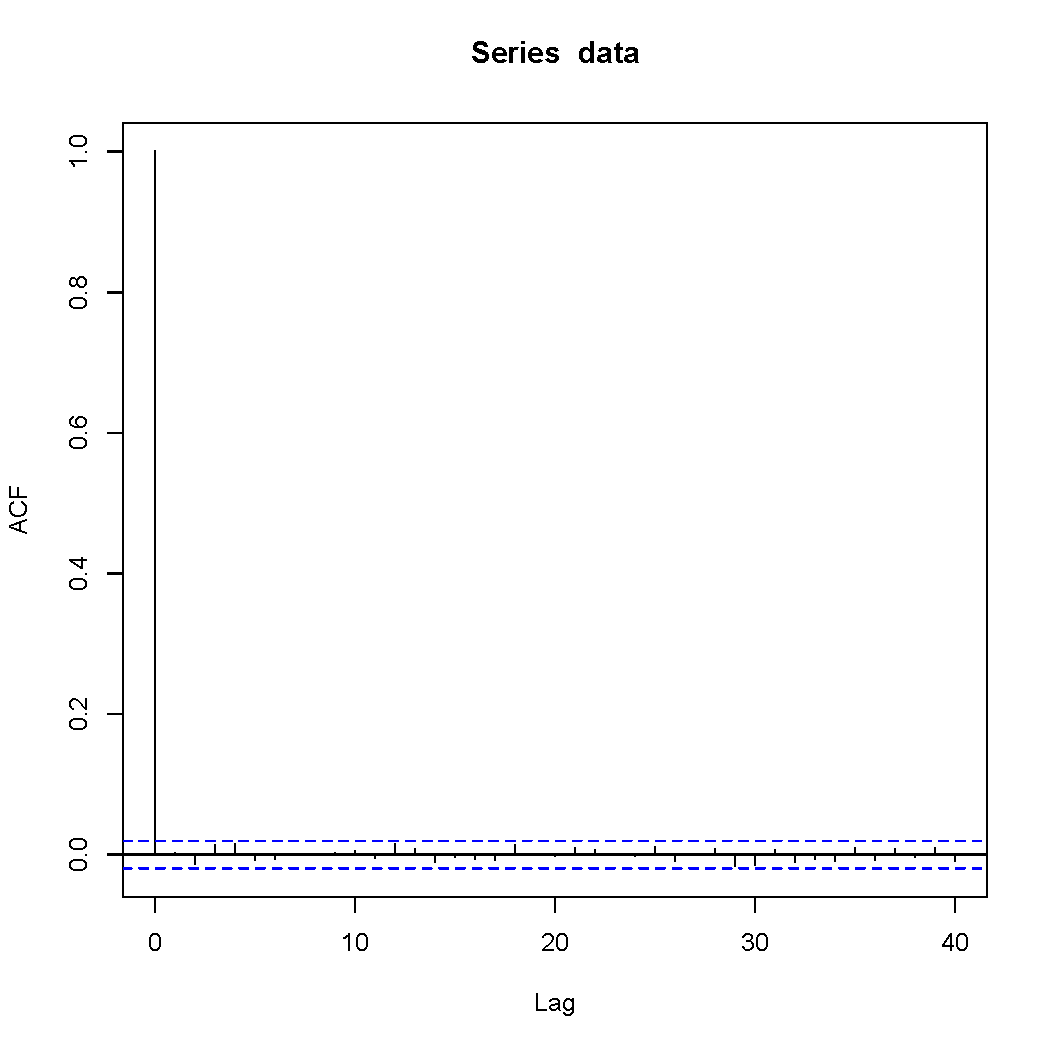
\includegraphics[scale=.42]{b4564acf.pdf}
\caption{ACF}
\label{fig:figure7}
\end{minipage}
\begin{minipage}[b]{0.45\linewidth}
\centering
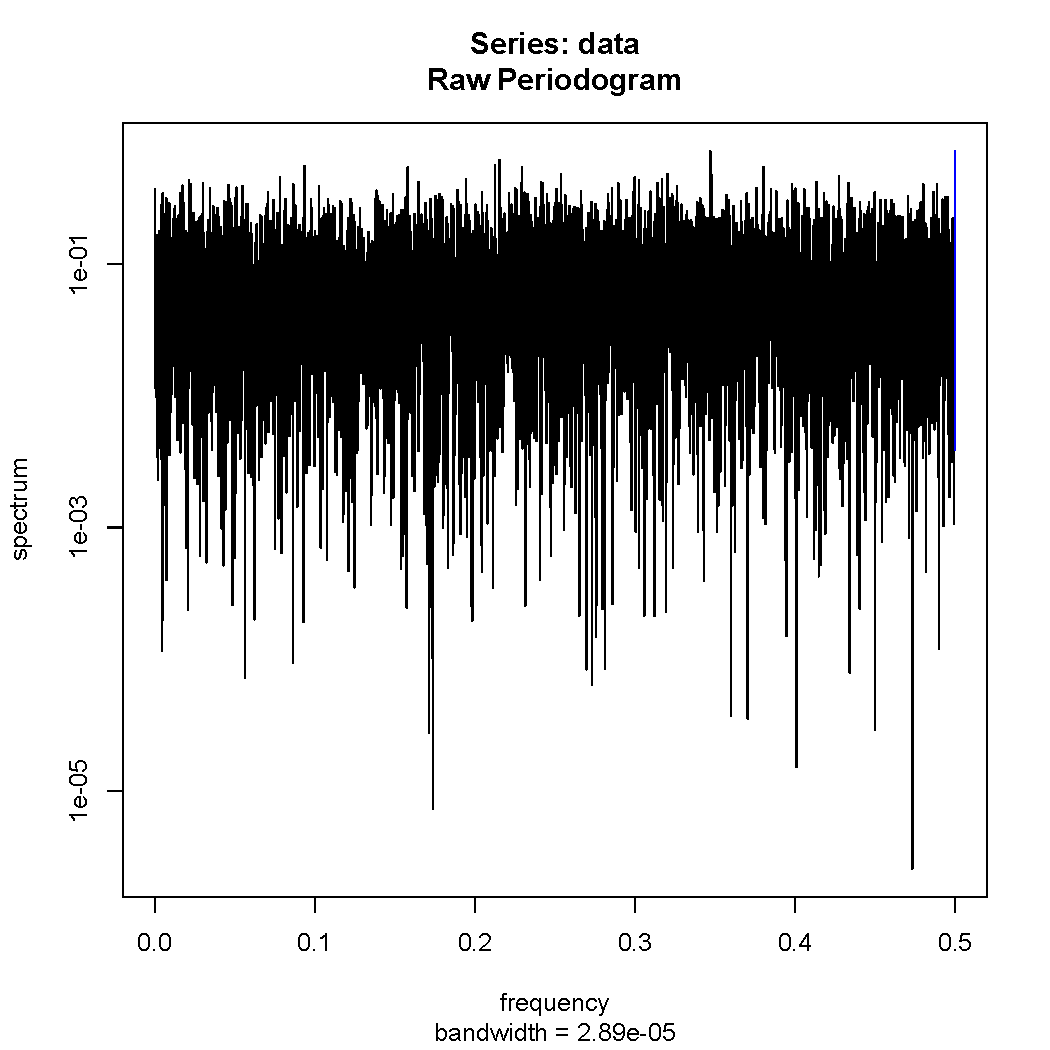
\includegraphics[scale=.42]{b4564pgram.pdf}
\caption{Periodogram}
\label{fig:figure8}
\end{minipage}
\end{figure}

\begin{verbatim}s1 = {7, 3, 2, 5, 4, 8, 9}, s2 = {4, 2, 7, 9, 5, 0, 6, 2, 3, 1, 5},
s3 = {5, 7, 4, 9, 8, 6, 2, 0, 1, 3, 6, 4, 2},
s4 = {1, 7, 9, 5, 0, 3, 2, 8, 4, 6, 0, 3, 4, 7, 9, 0, 5}\end{verbatim}

\newpage

Now that's better! We see that the mean and variance are almost exactly accurate, the raw data is pretty much uniformly distributed in its area, the CDF is almost exactly a straight line, and every lag on the ACF except 0 is minuscule and well within the confidence interval.  A comparison with the example in the second appendix, which contains an analysis of 10,000 uniformly distributed random variates from whatever algorithm R uses to generate random variables shows that our new generator seems to be just as good. 

By simply changing the length of the sequences of semi-arbitrary\footnote{
The sequences are slightly edited versions of the sequences from \texttt{nm1.c}, which were simply the digits 0-9 permutated according to my whimsey.}
digits, we have \emph{dramatically} improved the quality of the generator.  The sequence lengths were all prime (7, 11, 13, 17), and as such were all coprime to each other, and so created a period of $7*11*13*17 =  17,017$ for the added digits, an improvement of over 1700 orders of magnitude over our original period of 10.

Though the period of this generator is much better, it is still finite. We could potentially have a problem if we wanted to run long simulations, where periodic behavior from the random numbers would become noticeable even with long periods.  If we wanted to use this generator to run such a simulation, we may have to extend the sequences even further, but this is a small matter, as it would be trivial to implement and exactly as computationally efficient to have sequences of length 53, 59, 61, 67 (the first four prime numbers above 50), and we would get a period of 12,780,049.



%%%%%
%4
\newpage
\section{Conclusion}

$ $

The mid-square method, long abandoned by mathematicians and computer scientists, holds more potential than previously thought.  Though the original implementation of the algorithm was lacking in several ways, a few simple edits turned it into a pretty good generator.  It's statistical properties match the random number generator R provides, and it is computationally efficient.

The current standard in pseudorandom-number generation is Lehmer's linear congruential generator (LCG).  The second improved mid-square method (SIMM) described in this paper has both advantages and disadvantages to LCGs.  Unlike LCGs, subsequent terms should be independent of one another; I suspect that sequences of terms don't fall into a few hyperplanes.  However, the mid-square method lacks the precision of LCGs.  Since the maximum \texttt{long long} computable in C is 9,223,372,036,854,775,807 (18,446,744,073,709,551,615 for \texttt{unsigned long long}s, which is appropriate here), SIMM is operating near its maximum precision, which contains many fewer significant figures than that of an LCG.  However, I'm sure it's possible to mess around with the appended digits even more to allow for more precision, and the solution posed earlier in the paper (generate two four-digit variates $x_1, x_2$ and combine them to form $x_1x_2$) hold potential.  While at first glance a loss of synchronization is assured, we can use backshifting to obtain as many digits of precision as we want in the following way: generate two random variates $x_1, x_2$ and combine them to form our first final variate $x_1x_2$.  Generate a third random variate $x_3$, create $x_2x_3$ and repeat.  While we are using each four-digit variate twice, the reused variate is so small that it won't\footnote{Shouldn't, at least. I haven't investigated.} affect the statistical properties of the generator.  Essentially, we get double our digits for free.

In terms of future research, there are several things I'd like to investigate.  The first and foremost is dealing with the aforementioned lack of precision.  The technique I described above may actually affect the statistical properties, and we'd have to come up with something else.  It's possible that the algorithm could be altered simply (using fewer appended digits, including the lower-order appended digits, etc.) to increase the precision, but a more formal investigation than mere conjecture would be necessary.

I would also like to explore the sequences of appended digits more.  I came up with the existing sequences arbitrarily, and I'm sure there are some better ones to be used (we'll certainly need longer ones to increase the period).

I suspect the code I hacked out a few days ago is not totally efficient.  While it runs very quickly, I bet there's a better way than simply multiplying the appended digits by several million and adding them on to the seed.  Perhaps treating the digits as strings would be better, but string computation and conversion is usually slower than just arithmetic.  If the speed and efficiency could be increased, I really think this could become a legitimate generator.

It will also be necessary to do more statistical analysis.  While what I've done is relatively comprehensive, I haven't checked for runs at all and it's possible there's another Marsaglia out there who would ruin my fun.

Could this lead to a new standard in pseudorandom number generation? I certainly hope so, because I've always wanted to have my name on a math thing.

%%%%%
%5
\newpage
\section{Appendix I: Source Code}

%5a
\subsection{Original Mid-Square Method}

\begin{verbatim}/*
 * om.c                Robert Johns                April 29, 2014
 * This program generates 100 random variates (between 0 and 9999) by the mid-square
 * method in its orignal description by Jon von Neumann in 1949 (or Brother Edvin
 * between 1240 and 1250, depeding on your definition of "original"). 
 * Prints count and variate to track degenerance.
 */

#include <stdio.h>
#include <stdlib.h>

int main (int argc, char * argv[]) {
	
        	long count = 1;
        	long seed;
        	if (argc != 2) {
                 printf("usage: om [seed]\n");
                	exit(-1);
        	}
        	seed = atoi(argv[1]);
        	if (seed < 1 || seed > 9999) {
                	printf("error: seed must be between 1 and 9999\n");
                	exit(-1);
        	}
	
        	while (count < 100) {	
                 printf ("%4ld \t %ld\n", count, seed);
                 count++;
                	seed = (seed * seed) / 100 % 10000;
        	}
        	return 0;
}\end{verbatim}

%5b
\newpage
\subsection{First Improved Method}

\begin{verbatim}/* 
 * nm1.c		Robert Johns		April 29, 2014
 * This program generates random variates (between 0 and 9999) by the first attempt
 * at an improved midsquare method as described by Robert Johns in the final project
 * for CSCI 678: Statistical Analysis of Simulation Models in the Spring 2014 term
 * at William & Mary.  
 */

#include <stdio.h>
#include <stdlib.h>

int main (int argc, char * argv[]) {
	
        	long 	  count;
        	long 	  max;
        	long long seed;
        	long long seq1[] = {7, 3, 2, 5, 4, 8, 9, 0, 1, 5};
        	long long seq2[] = {4, 2, 7, 9, 5, 0, 6, 2, 3, 1};
        	long long seq3[] = {5, 7, 4, 9, 8, 6, 2, 0, 1, 3};
        	long long seq4[] = {1, 7, 9, 5, 2, 3, 2, 8, 4, 6};
	
        	if (argc != 3) {
                	printf("usage: nm1 [seed] [max]\n");
                	exit(-1);
        	}
	
	
        	seed = atoll(argv[1]);
        	max = atol(argv[2]);
	
        	if (seed < 1 || seed > 9999) {
                	printf("error: seed must be between 1 and 9999\n");
                	exit(-1);
        	}
	
        	count = 0;
        	printf ("%lld\n", seed);
        	count++;
        	while (count < max) {
		
                	seed = seed * 100;
                	seed += (10 * seq1[count % 10] + seq2[count % 10]);
                	seed += (10000000 * seq3[count % 10] + 1000000 * seq4[count % 10]);
                	seed = ((seed * seed) / 1000000) % 10000;
                	printf ("%lld\n", seed);
                	count++;	
        	}
        	return 0;
}\end{verbatim}

%5c
\newpage
\subsection{Second Improved Method}

\begin{verbatim}/* 
 * nm2.c		Robert Johns		April 29, 2014
 * This program generates random variates (between 0 and 9999) by the second attempt
 * at an improved midsquare method as described by Robert Johns in the final project
 * for CSCI 678: Statistical Analysis of Simulation Models in the Spring 2014 term
 * at William & Mary.
 */

#include <stdio.h>
#include <stdlib.h>

#define SEQ1LEN 7
#define SEQ2LEN 11
#define SEQ3LEN 13
#define SEQ4LEN 17

int main (int argc, char * argv[]) {
	
        	long 	  count;
        	long 	  max;
        	long long seed;
        	long long seq1[] = {7, 3, 2, 5, 4, 8, 9};
        	long long seq2[] = {4, 2, 7, 9, 5, 0, 6, 2, 3, 1, 5};
        	long long seq3[] = {5, 7, 4, 9, 8, 6, 2, 0, 1, 3, 6, 4, 2};
        	long long seq4[] = {1, 7, 9, 5, 0, 3, 2, 8, 4, 6, 0, 3, 4, 7, 9, 0, 5};
	
	
        	if (argc != 3) {
                	printf("usage: nm2 [seed] [max]\n");
                	exit(-1);
        	}
	
        	seed = atoll(argv[1]);
        	max = atol(argv[2]);
	
        	if (seed < 1 || seed > 9999) {
                	printf("error: seed must be between 1 and 9999\n");
                	exit(-1);
        	}
	
        	count = 0;
        	printf ("%lld\n", seed);
        	count++;
        	while (count < max) {
		
                	seed = seed * 100;
                	seed += (10 * seq1[count % SEQ1LEN] + seq2[count % SEQ2LEN]);
                	seed += (10000000 * seq3[count % SEQ3LEN] + 1000000 * seq4[count % SEQ4LEN]);
                	seed = ((seed * seed) / 1000000) % 10000;
                	printf ("%lld\n", seed);
                	count++;
		
        	}
	return 0;
}\end{verbatim}

%5d
\newpage
\subsection{Statistical Tests}

\begin{verbatim}# rngTests.r        Robert Johns        April 29, 2014
# scans a sequence of random variates valued between
# 0 and 9999 and runs statistical analysis on them 
# to check that they are indeed uniformly distributed
# and that they are sufficiently random.

# get data and compress to [0,1]
data = scan("data.txt")
data = data / 10000

# print seed, mean, variance
print(data[1])
print(mean(data))
print(var(data))

# plot raw data, cdf, autocorrelation function, periodogram
plot(data, pch = '.')
sdata  = sort(data)
plot(sdata, pch = '.')
abline(h = mean)
acf(data)
spec.pgram(data)\end{verbatim}

%6
\newpage
\section{Appendx II: Analysis of R's Pseudorandom Number Generator}

Generating 10,000 variates with R's Pseudorandom Number Generator (assumed to be an LCG)

Mean: 0.4990327, variance: 0.08352679, max: 0.999767, min: 9.462563e-05

\begin{figure}[ht]
\begin{minipage}[b]{0.45\linewidth}
\centering
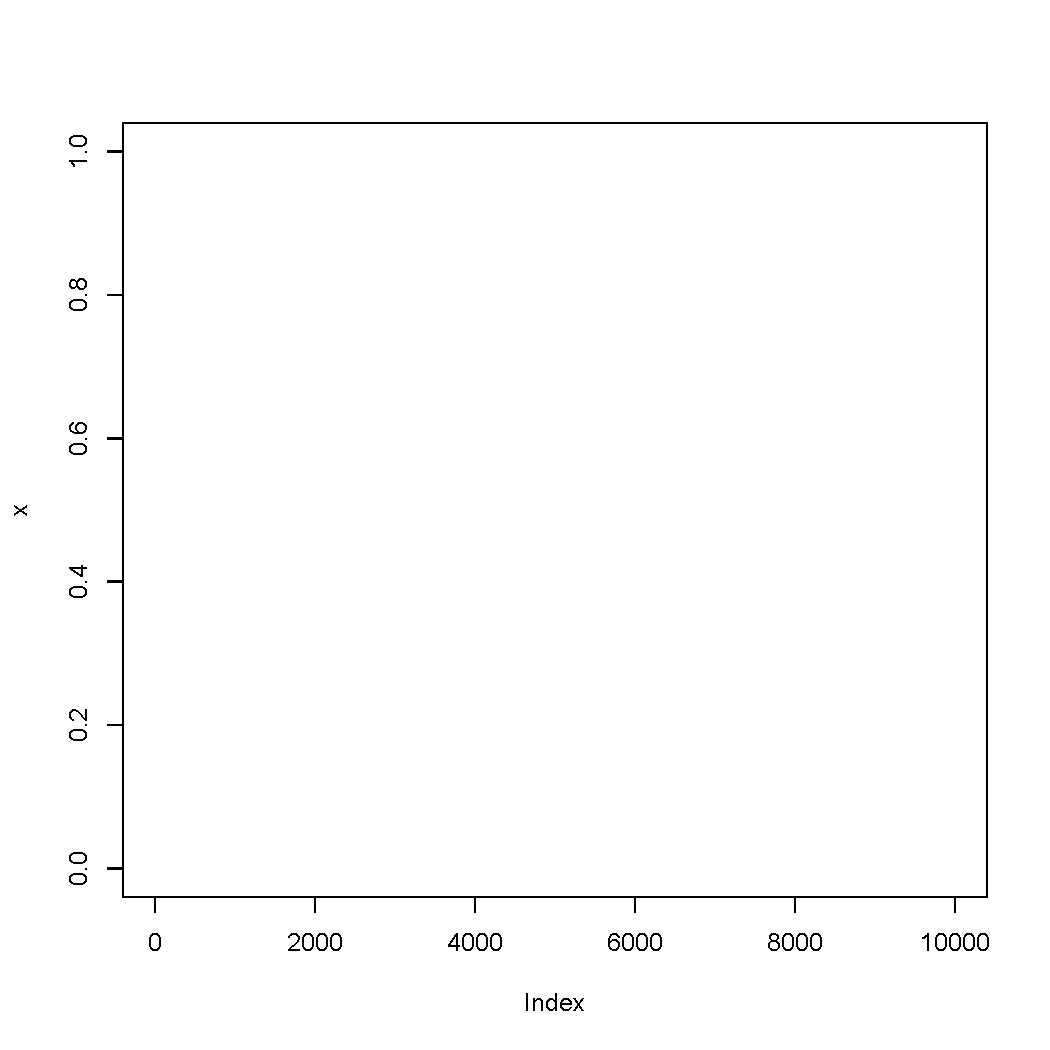
\includegraphics[scale=.42]{rRaw.pdf}
\caption{Raw data}
\label{fig:figure1}
\end{minipage}
\begin{minipage}[b]{0.45\linewidth}
\centering
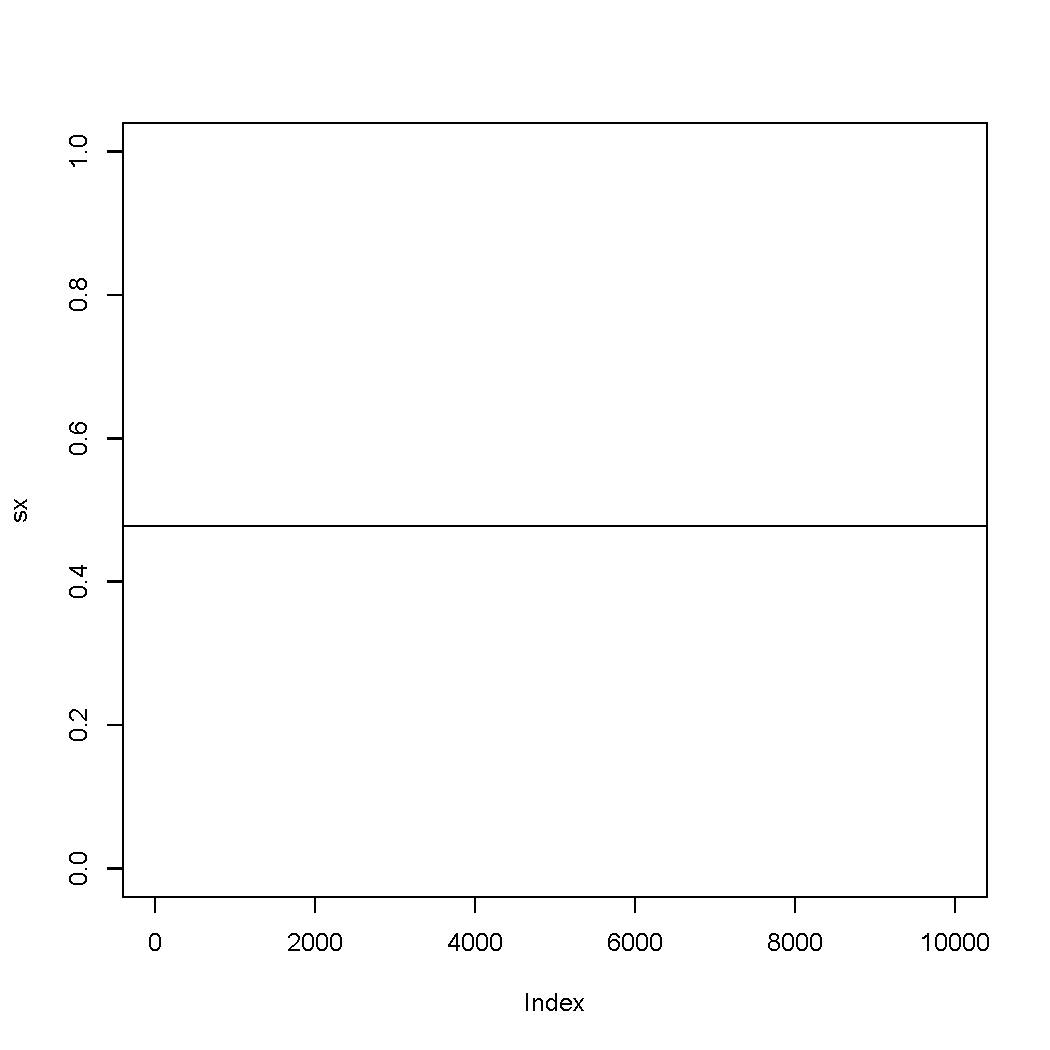
\includegraphics[scale=.42]{rCDF.pdf}
\caption{CDF with mean line}
\label{fig:figure2}
\end{minipage}

\begin{minipage}[b]{0.45\linewidth}
\centering
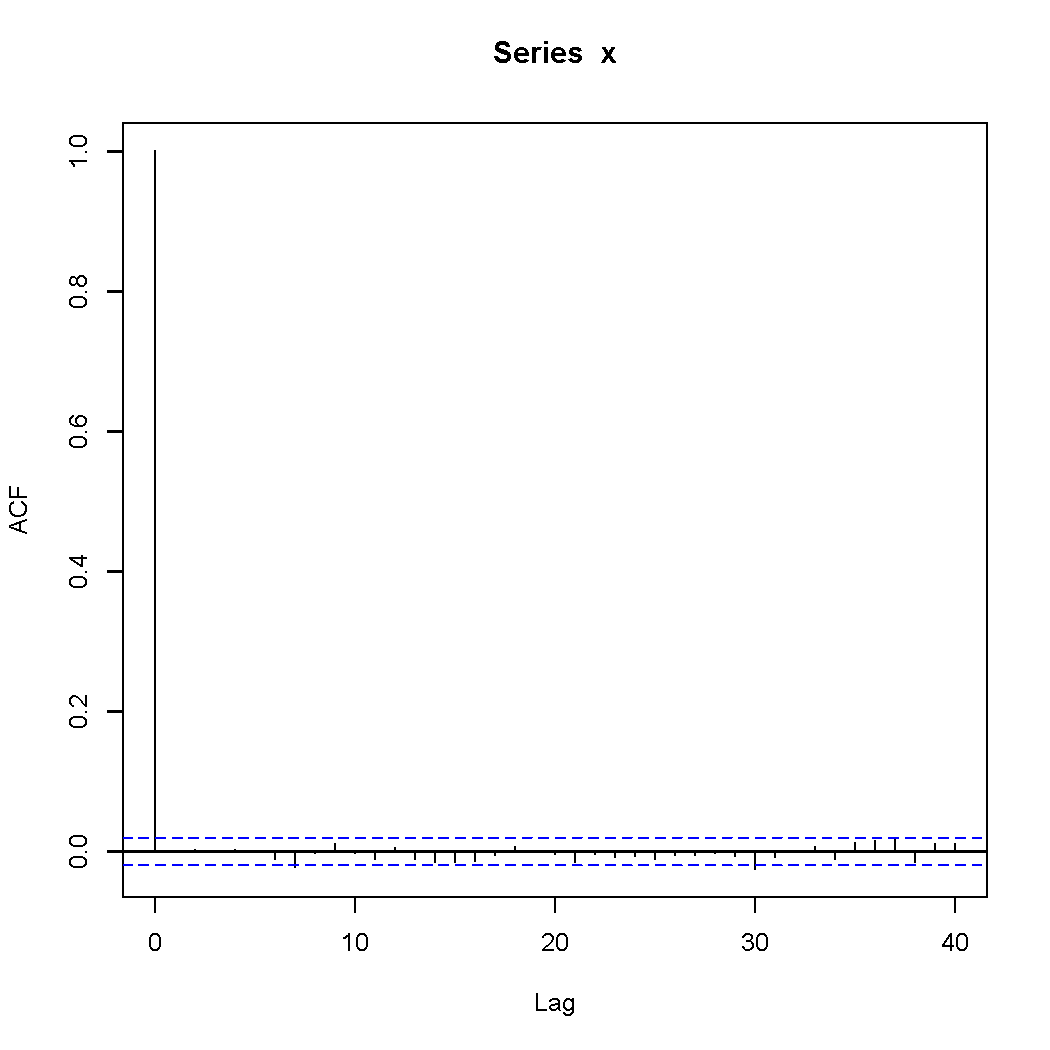
\includegraphics[scale=.42]{rACF.pdf}
\caption{ACF}
\label{fig:figure3}
\end{minipage}
\begin{minipage}[b]{0.45\linewidth}
\centering
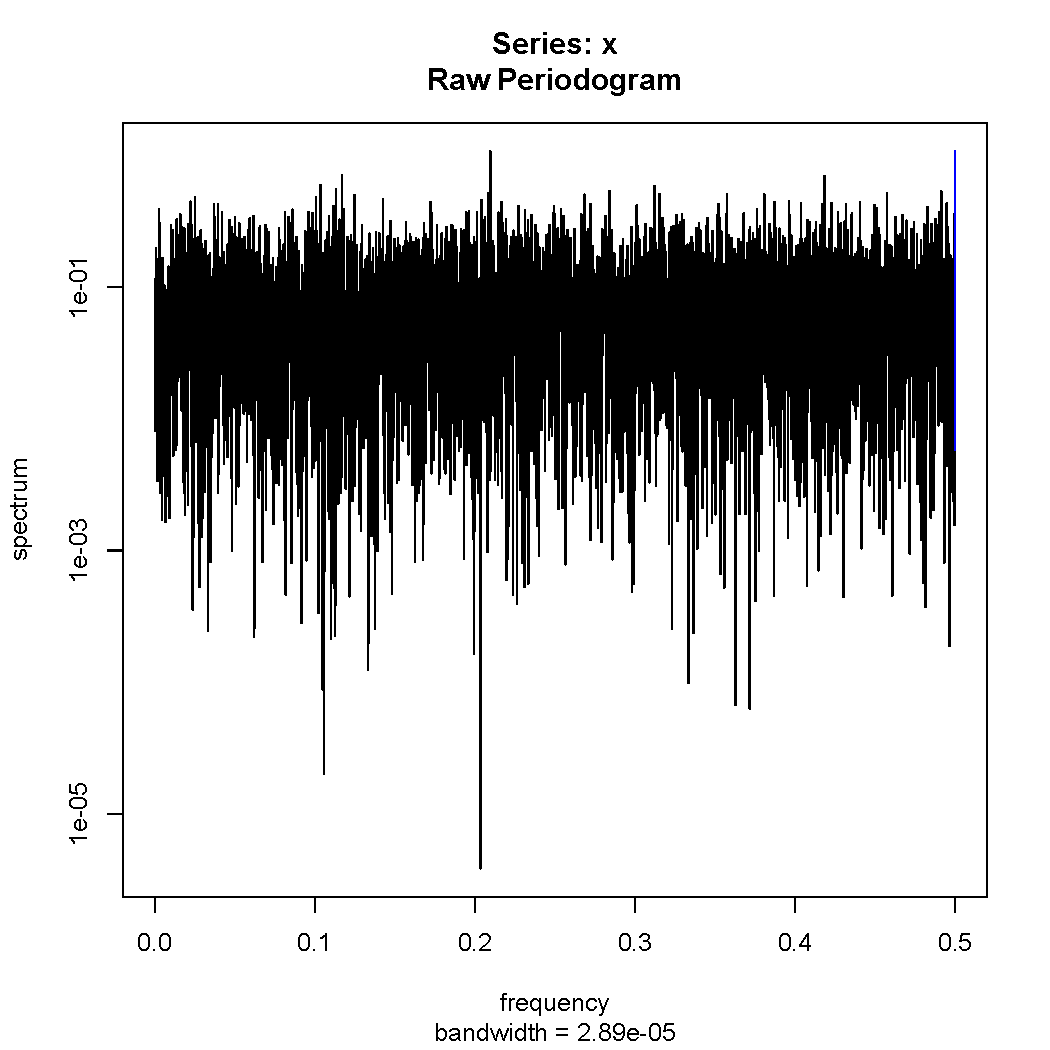
\includegraphics[scale=.42]{rPgram.pdf}
\caption{Periodogram}
\label{fig:figure4}
\end{minipage}
\end{figure}

\end{document}